% !TeX root = ../main/thesis_main.tex
% ---------------------------------------------------
% ----- Chapters of the template
% ----- for Bachelor-, Master thesis and class papers
% ---------------------------------------------------
%  Created by C. Müller-Birn on 2012-08-17, CC-BY-SA 3.0.
%  Freie Universität Berlin, Institute of Computer Science, Human Centered Computing.
% 
% Set up python path for all used code in this session and track all external files
\begin{pycode}
import sys
sys.path.insert(0, '../chapters/implementation/code/')
# track code

\end{pycode}

\chapter{Implementation}
\label{chap:implementation}

\section{General setup}

In order to ensure that the results of this thesis are usable for further work and research it was one of my priorities to integrate all my code into the existing project as well as possible. Since the IKON project uses a Docker-based microservice architecture to develop and manage their servers, I decided to integrate the Jupyter Notebook, which I used as my main tool for code development and documentation, into this network. Doing this also enabled the Notebook to dynamically fetch data from the Postgres database which serves as the main source of information.
In anticipation of huge computational loads the Docker container was designed to make use of a potential graphic card. That's why I built all my work on top of the official Tensorflow Docker image which comes with all the drivers for NVidia GPUs. The problem with that image is that it either detects a graphic card and suitable drivers and works or it fails in case of no present drivers. For that reason I created a Shell which makes the use of the container easier. By activating a $--gpu$ flag while executing the script, the docker container dynamically selects an image with or without GPU support, starts the Notebook container and the database in a separate network and scans the output of the Notebook container in order to extract the Notebook credentials, which are necessary to access the program via the browser, and opens a browser session once these credentials were found.

\section{Data and Preprocessing}
Since one of the main aims of project IKON is to connect projects semantically instead of by using the rigid taxonomy of the museum, I was able to use the project's abstract which is recorded in the GEPRIS database of the DFG \cite{DFGGEPRIS}. It consists of almost all projects which were supported by the DFG since 2000. Fortunately, another bachelor project before me worked on a scraper which extracted approximately 114.000 projects from the web interface of the database since there is no publicly available API. Each project was characterized by a title, a project abstract in German or English, start and end dates as well as additional meta data like connected institutions or people working in the project.

As one can see in \autoref{pic:gepris_histogram}, there is a peak at word count 3 and one at approximatly 100. The first one corresponds to all projects which do not have descriptions, because they are described with "Keine Zusammenfassung vorhanden". The latter peak on the other hand is produced by projects from a fund which uses the same descriptions for all its projects which are financed through the DFG.

\begin{figure}[t]
	\centering
	\includegraphics[width=400px]{/home/tim/HCC/IKON-backend/src/topicextraction/nlp/plots/histogram}
	\caption{\label{pic:gepris_histogram} Histogram showing the distribution of text lengths in the dataset}
\end{figure}

Removing these peaks in \autoref{pic:gepris_cleaned_histogram} reveals that most texts have an length of 150 words, while also having smaller peaks at ca. 70 and 350 words. The shortest description has a length of one word and the longest  983 words.

\begin{figure}[t]
	\centering
	\includegraphics[width=400px]{/home/tim/HCC/IKON-backend/src/topicextraction/nlp/plots/cleaned_histogram}
	\caption{\label{pic:gepris_cleaned_histogram} Histogram showing the distribution of text lengths in the dataset excluding duplicates and projects without a description}
\end{figure}

Following the advice of Matthew et al. \cite{dennymatthewpennstateuniversity;spirlingarthurnewyorkuniversityReplicationDataText2017} the texts were preprocessed by a P-N-S-W scheme. First punctuation (P) and numbers (N) were removed since sentence boundaries or specific numbers do not bear a lot of information in middle-sized descriptive texts. Following this, according to the categories of Matthew et al., a stemming step (S) is performed, which uses lemmatization to find the lemmas of words by using vocabularies and the context of each word. The last step removes infrequent words without much semantic meaning, commonly known as stopwords (W). Lowercasing and n-gram inclusion were omitted, because casing is an important feature for distinguishing nouns from other word types in the German language, which helps the lemmatization step, and the use of word composition makes most reasonable n-grams in other languages appear as one word in German. 

Until the start of this thesis the pipeline did all this preprocessing using regex-based rules and a lemmatization using the SpaCy lemmatizer. This proved to be a viable option until a corpus size of 5000 since after that point the running time was too long to effectively work with it. Therefore I bundled all the preprocessing operations in a new class called \textit{Datapreprocessor}, which should be able to transform any given query into a preprocessed dataset for the following pipeline steps as well as cache its results. In order to do that I rewrote the preprocessing steps and integrated them into the already existing SpaCy pipeline which uses a CNN to apply the previously discussed preprocessing. Additionally it is able to detect the language of a text, which, in turn, makes it possible to filter out all non-German texts. Using this existing framework gave me the opportunity to embed my custom code into the Cython code of the framework accelerating the looping over the corpus. Additionally I was able to fully parallelize the process on $n$ CPUs by splitting the corpus in $n$ chunks and feeding each chunk into a separate sub-process to make use of the batch sizes of the SpaCy neural networks. This accelerated the preprocessing by a factor of 10.

\section{The existing pipeline}

The existing pipeline was implemented by me as a proof-of-concept for project \textit{IKON}. Following the structure of \autoref{pic:general_topic_extraction_pipeline} the first step is a document vectorization of the given texts in order to embed them in one common vector space. One of the simplest and still effective methods is a Tf-Idf Bag-Of-Words (TfIdf-BOW) embedding. With this procedure each text is represented as a set of terms, the bag of words. Having a whole corpus it is now possible to assign a vector to each document $D$ in corpus $C=\{D_1, ..., D_n\}$ of length $N = |C|$, where each entry $i$ is the number of term occurrences of term $t_i$ in $D$. That means that each document gets embedded into a vector space of dimensionality $|(\text{unique terms in C})|$ and the corpus becomes a matrix of size $|(\text{unique terms in C})| \times N$. In order to additionally introduce information from the whole corpus into each vectorized document and therefore contextualize it, each entry is replaced by $C_{t,d}=Tf(C_{t,d}) \cdot Idf(C,t,d)$ where $Tf(t,d)$ is often the identity function and $Idf(C,t,d)$ is $\log\frac{N}{|\{ D \in C : t_t \in D \}|}$. \cite{PivotedDocumentLength} The notion behind this is intuitive. The higher the term frequency of a term in a document, the more important it is for this specific document and the more a term appears in several documents, the less it caries information to seperate a document from others. \tk{Needs maybe rework based on Shannon theory} This ensures that words which are specific to a small group of documents and appear often in them, get a higher weight, while terms which are infrequent or too frequent in many documents, as articles for example, get a small weight.

Now that we have a vector representation of each document, we could work in the existing space and try to cluster our documents in their current form using k-Means, which will be explained later. An exemplary analysis shows that the semantic coherence of the document clusters seems to lack. \tk{show proof} That is due to the clustering algorithm failing to perform and facing, what is commonly known as, \textit{the curse of dimensionality}. The curse of dimensionality states for distance based methods that "under certain reasonable assumptions on the
data distribution, the ratio of the distances of the nearest and farthest neighbors
to a given target in high dimensional space is almost 1 for a wide variety of data
distributions and distance functions" \cite{aggarwalSurprisingBehaviorDistance2001}. Therefore closeness between points, which is the relevance metric for the k-Means algorithm due to it using the Euclidian distance, becomes effectively meaningless and making it necessary to reduce the dimensionality of the vector space.

One popular method, which is often used in conjunction with Tf-Idf BOW embeddings, is the Latent Semantic Indexing (LSI), also known and henceforth referenced as Latent Semantic Analysis (LSA). A LSA operates on the premise that a vectorized corpus contains latent structures, which my correspond to topics for example. Such a topic would consist of several words which are semantically connected and therefore appear together more often than words which are not semantically similar. Adding constraints such as adjustable representational richness, which depicts sufficient parameterisation, explicit representation of both terms and documents and computational tractability for large datasets the authors decided to use a Singular Value Decomposition (SVD) \cite{deerwesterIndexingLatentSemantic}. The SVD is closely related to Principal Component Analysis (PCA) and reduces the dimensionality of a dataset by removing the dimensions with the least variance, effectively projecting the vector space onto the subspace with the highest variance and therefore the most information contained. Applying a SVD on the corpus changes the representation of the document from being a linear combination of words into being a linear combination of latent topics. This representation is now usable for most other methods such as clustering due to its smaller dimensionality. The existing pipeline uses a k-Means algorithm to discover clusters and classify the documents as a next step. Finally, in order to visualize the high dimensional topic space in 2D a linear discriminant analysis is used using the clustering as labels.  \tk{Connections to BPMN}


\section{Document embedding}

\subsection{A short survey of document embedding techniques}
Since 1972, the year when the Idf measure was proposed for the first time, \cite{robertsonUnderstandingInverseDocument2004} a number of other techniques appeared, which are able to vectorize documents in a corpus.

Another popular technique was published by Blei et al. \cite{bleiLatentDirichletAllocation2003} in 2003. \textit{Latent Dirichlet Allocation} is a hierarchical Bayesian model, which describes documents as a finite mixture of latent topics, while topics are an infinite mixture of latent topic probabilities. The LDA therefore performs the embedding and the topic extraction step at once.

Le and Mikolov \cite{leDistributedRepresentationsSentences2014} proposed \textit{Paragraph vectors} almost a decade later using the newest advances in neural networks. This technique, also known as \textit{Doc2Vec}, because it expands the idea of Word2Vec \cite{mikolovDistributedRepresentationsWords} to documents, utilizes a shallow neural network to run over each document with a sliding window and predict a token in this window using the other tokens and a paragraph id as a special token as context. Using a standard backpropagation algorithm to train the weights of the network the final paragraph vector consists of the weights which are used for the paragraph id. The intuition is that the paragraph vector acts as an additional storage for context information and since the connected paragraph ID is unique for each document it contains semantic information for the entire document. Choosing a low dimension as an embedding dimension also corresponds to the embedding and topic extraction step at once, but the authors recommend an embedding dimensionality of at least 100.

A rather new method was presented by Wu et al. \cite{wuWordMoverEmbedding2018} using a new distance metric called \textit{Word Mover's distance}(WMD). This metric uses pretrained word vectors and word alignment in order to compute more meaningful distances. Because the computation of this metric is quite expensive, Wu et al. develop an approximative kernel which embeds a corpus into a vector space using the WMD, which can be used instead of computing the full kernel with all the training data.

Another approach would be to not train a model on the specific dataset, but rather use a model which was pretrained on a huge and very general dataset. One of the state-of-the-art techniques for that is BERT \cite{devlinBERTPretrainingDeep2018}. Devlin et al. present a new model architecture based on the popular Transformer model \cite{vaswaniAttentionAllYou2017} and train it in the first version on a concatenated corpus of BookCorpus and the English Wikipedia ($3,3\cdot 10^9$ words in total).  Having such a huge amount of data as context knowledge one is now able to train another model for downstream tasks on top of BERT and utilize the knowledge extracted from the corpus in a transfer learning fashion. It is also possible to extract the raw document embeddings from BERT directly, but the sequence length is capped to 512 characters.

\begin{figure}[t]
	\centering
	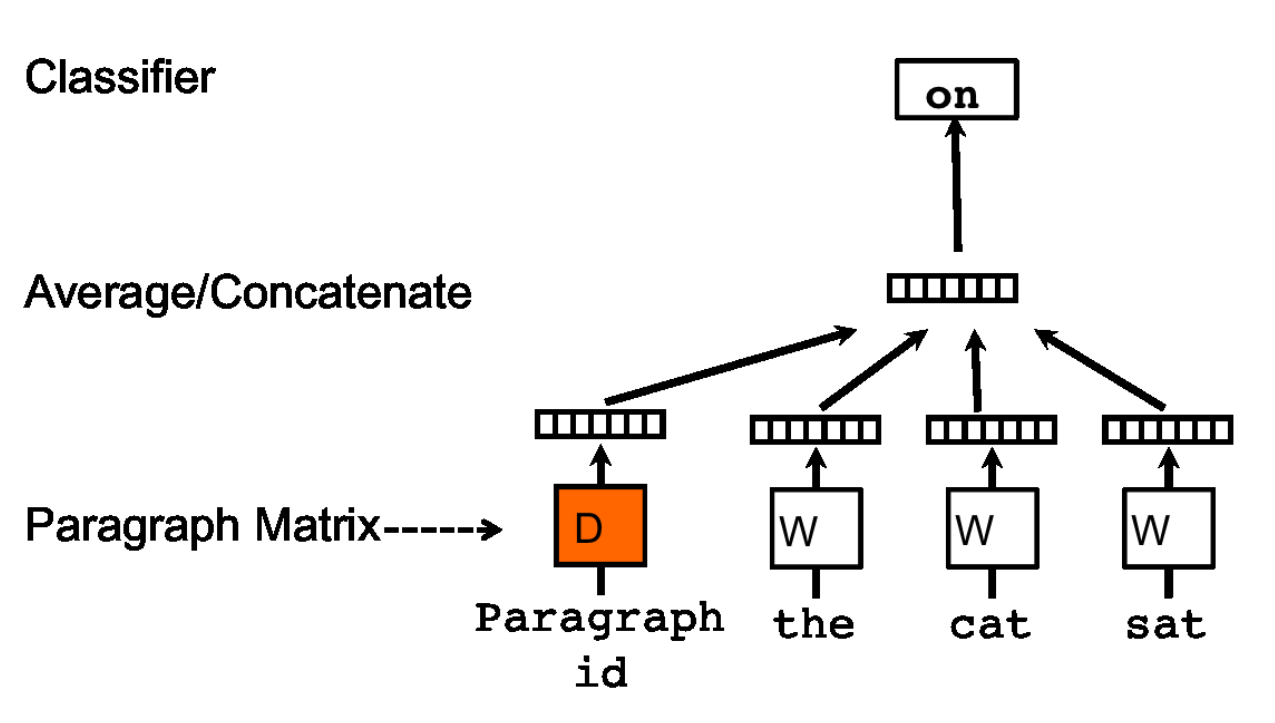
\includegraphics[width=250px]{../chapters/implementation/pics/doc2vec}
	\caption{\label{pic:doc2vec} Visualization of a training step of a Doc2Vec network {\cite{wuWordMoverEmbedding2018}}}
\end{figure}

\subsection{Selection of a document embedding technique}

Summarizing the previously discussed methods by three of their main characteristics - number of hyperparameters, maximum processable document length and type of model results in  \autoref{tab:overview_doc_embedding}.
\begin{table}
	\centering
	\begin{tabular}{ c | c | c }
		\hline 
		Technique & Max. document length & Type \\ \hline
		Tf-Idf BOW & unlimited & Probabilistic \\ \hline
		Latent Dirichlet Allocation & unlimited & Probabilistic \\ \hline
		Doc2Vec & unlimited & NN \\ \hline
		Word mover's embedding & unlimited & Kernel method \\ \hline
		BERT & 512 characters & NN \\ \hline
	\end{tabular}
	\caption{\label{tab:overview_doc_embedding} Table summarizing the key features of different document embedding techniques}
\end{table}

The model is now selected by exclusion. Since our database contains documents which are longer than 512 tokens and each token has a length of at least 1 character, BERT is eliminated as a potential document embedding technique. It would be possible to take word embeddings from BERT and average them in order to get a document embedding as it was proposed and further developed in \cite{deboomRepresentationLearningVery2016} for Word2Vec embeddings, but there was no scientific or non-scientific literature that suggested that this works for the case of BERT embeddings. \tk{Why is BERT different?}
Furthermore the previous literature analysis showed that there is not a lot of work done for explaining probabilistic models or models utilizing kernel tricks, therefore TF-Idf BOW, the LDA and the Word Mover's embedding are not of interest in this case. Only Doc2Vec remains, supporting both an unlimited document length and being of type 'NN' and therefore potentially being able to support more explainability techniques which may be developed in the future.

\subsection{Explainability technique: Top words}

Looking at \autoref{fig:pipelinestep_gamut} shows that local instance explanations as a strategy to explain the output of an unsupervised embedding algorithm are most prevalent among all sourced publications. Factoring in the two questions from \autoref{tab:overview_viz_questions} which deal with the most prominent topics and the similarity between projects and clusters I will rank the input features to the document embedding and topic extraction step for each document and cluster. 

Assume that I have a document described as a vector $c \in \mathbb{R}^k$ in the latent topic space. In order to show the most important features in the document the idea is to go backwards. Taking the vector in the latent space firstly the inverse dimensionality reduction is applied in order to transform the vector into the embedding space. Both the LSA and the autodecoder approach have this opportunity, but they differ greatly in quality of this reconstruction. Since the LSA is a linear method, the back projection yields all documents on a hyperplane, while the autodecoder is able to minimize the reconstruction loss through its inherent nonlinearity. 

Now that the document vector is in its embedding space we will make use of a special ability of the Doc2Vec model. As described in the previous section the model does not only train document vectors, but it also generates word embeddings in the same space. The revolution the Word2Vec model, as a base of the Doc2Vec model, presented was that the generated embeddings and their relations to eachother encoded semantic relations. Although there is no literature on this, it is a hypothesis that this behaviour also applies to the embedding of document and word vectors into one space. This leads to the possibility of describing a document by its nearest word vectors. An exemplary analysis shows that there seems to be a valid semantic structure in the relations between tokens and between tokens and documents. As a German native speaker it is easy for me to verify that the word queries in \autoref{tab:semantic_connectivity_words} are indeed semantically well connected. The results of the document queries in \autoref{tab:semantic_connectivity_docs} on the other hand are hard to verify since most documents are very specific, scientific texts. I picked two projects and their top words which I was able to understand without relying on external information. The first three top words are indeed well connected to the topic of the corresponding project, but the last two ones seem to be off. This exemplary analysis speaks in favor of the hypothesis that there are indeed semantic connections document vectors and word vectors.

\begin{table}
	\centering
	\begin{tabular}{ p{6cm} | p{6cm} }
		"Evolution" & "Diversität" \\ \hline
		\begin{enumerate}
			\item evolutionären
			\item evolutionäre
			\item evolutionärer
			\item phylogenetische
			\item Artbildung
		\end{enumerate} & 
		\begin{enumerate}
			\item Artenzusammensetzung
			\item Biodiversität
			\item Taxa
			\item taxonomisch
			\item Lebensräumen
		\end{enumerate} \\
	\end{tabular}
	\caption{\label{tab:semantic_connectivity_words} Table showing the top five similar words for two queries by word}
\end{table}

\begin{table}
	\centering
	\begin{tabular}{ p{6cm} | p{6cm} }
		\href{https://gepris.dfg.de/gepris/projekt/387798678}{'Ambitionierte Amateure' - Europäische Filmclubs in den langen 1960er Jahren} & \href{https://gepris.dfg.de/gepris/projekt/160874660}{Netzwerke im europäischen Handel des Mittelalters} \\ \hline
		\begin{enumerate}
			\item Kulturpraxis
			\item Kulturzentren
			\item alltagsweltlich
			\item pain
			\item Ceuta
		\end{enumerate} & 
		\begin{enumerate}
			\item Opportunitätskosten
			\item Diskursteilnehmer
			\item evoluieren
			\item schloss
			\item Staphylococcen
		\end{enumerate} \\
	\end{tabular}
	\caption{\label{tab:semantic_connectivity_docs} Table showing the top five similar words for two queries by document}
\end{table}

Keeping the gist of this strategy the first explainability technique I propose id the \textit{Top words} method.

\section{Topic extraction}

Currently the only used topic extraction method is the LSA. Since the underlying SVD is a purely linear technique, the questions stands if the results of the topic extraction improve when nonlinear features are taken into account. One technique to perform an nonlinear, unsupervised dimensionality reduction is the \textit{Autoencoder}. This type of neural network consists of an encoder network and a decoder network as seen in \autoref{pic:autoencoder}. The encoder maps an input to an intermediate layer, while the decoder maps a vector from its representation in the intermediate layer to a vector in the vector space of the original input.

The composition of encoder and decoder is then trained to reconstruct the input from its intermediate layer via a standard backpropagation algorithm. Choosing the intermediate layer of lesser dimensionality compresses the input vectors, which constitutes as a dimensionality reduction. As Wang et al. \cite{wangAutoencoderBasedDimensionality2016} pointed out, an autoencoder can emulate the results of a PCA/SVD by choosing a linear activation function for all neurons and may even outperform it for other nonlinear activation functions.

Adding a sparsity constraint to the encoding network can help to describe a project by as little features as possible. Since the features could be interpreted as topics, this constraint helps the clustering task downstream.

\begin{figure}[t]
	\centering
	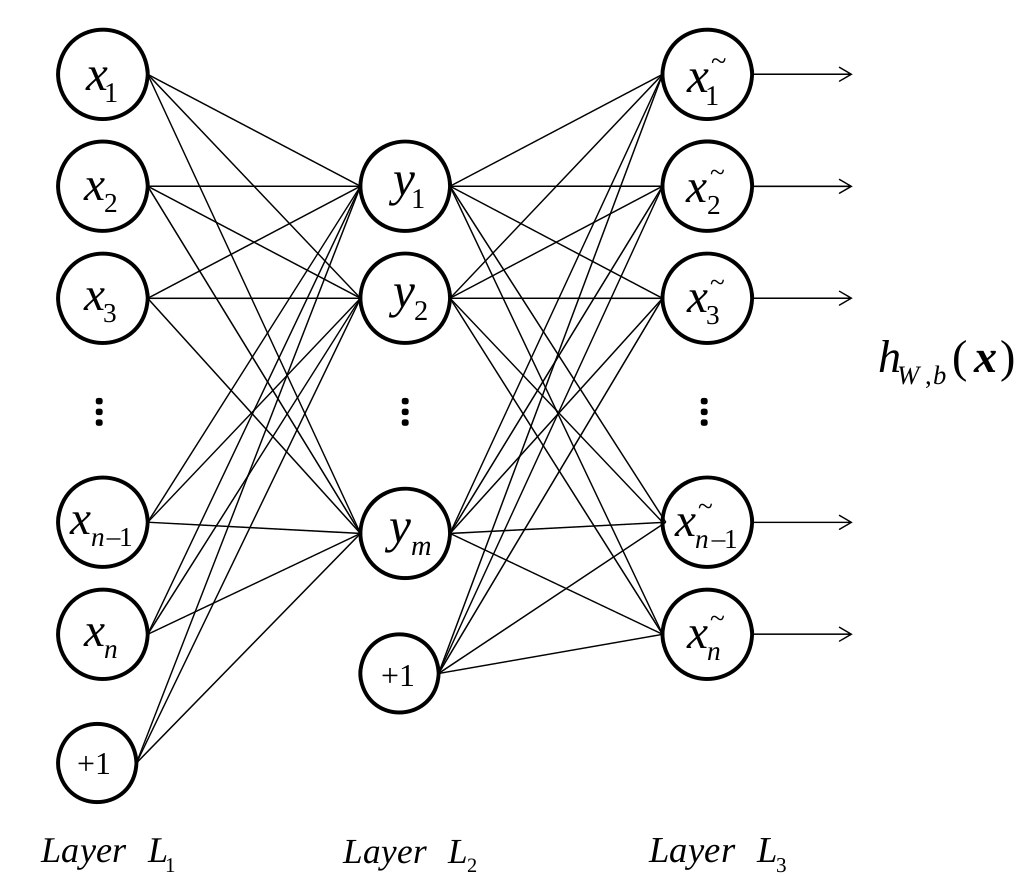
\includegraphics[width=250px]{../chapters/implementation/pics/autoencoder}
	\caption{\label{pic:autoencoder} Strucuture of a simple autoencoder {\cite{wangAutoencoderBasedDimensionality2016}}}
\end{figure} 

Training the model with an embedding dimension of 50, binary crossentropy as a loss function and Adadelta optimizer shows that the model achieves a loss of 0.005 after 75 epochs on the training set and approximately 0.01 on the validation set \autoref{pic:autoencoder_loss}.

\begin{figure}[t]
	\centering
	\includegraphics[width=400px]{/home/tim/HCC/IKON-backend/src/topicextraction/nlp/plots/autoencoder_loss}
	\caption{\label{pic:autoencoder_loss} Graph showing the training and validation loss of the autoencoder over progressing epochs}
\end{figure}

 

\section{Clustering}

As described in the beginning of this chapter a K-Means clustering would now classify the documents in the latent topic space. A problem that this approach poses is that the assumption that the Euclidian distance (EuD), which is the inert similarity measure of the K-Means algorithm \tk{Cite!} is meaningful in our vector space may not be true. \tk{Cite?} Another distance measure which may may encode more semantic meaning could be the previously mentioned \textit{Word Mover's Distance}. Since it uses the generated word embeddings and their order in the document to compute distances, it may be more suited for comparing texts and subsequently also yield better results for the clustering. This weighs even heavier if the corpus is vectorized as a sparse matrix since the Euclidian distance, as described in \autoref{chap:introduction}, looses its meaning . In our case, having embeddings from a Doc2Vec model, we don't have to deal with this additional problem, but the question remains if the two distance measures differ on our dataset.  
Comparing the distances between documents generated by both the Word Mover's distance and the Euclidian distance in \autoref{pic:wmd_eud_boxplot} it is apparent that there is indeed a difference. Therefore it is worth investigating if using this information improves the clustering results. 

\begin{figure}[t]
	\centering
	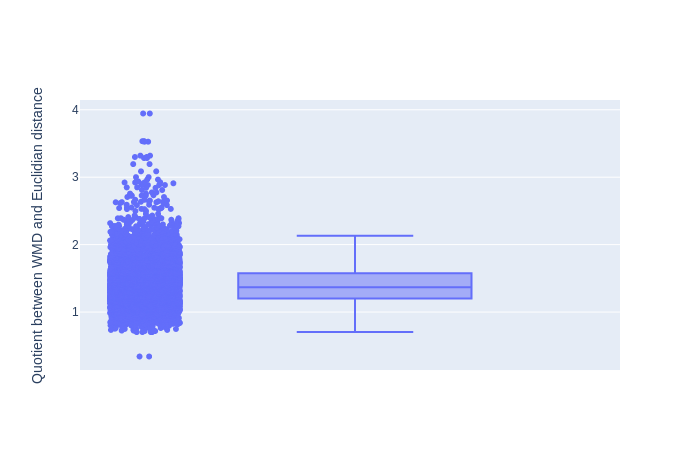
\includegraphics[width=400px]{/home/tim/HCC/IKON-backend/src/topicextraction/nlp/plots/wmd-eud}
	\caption{\label{pic:wmd_eud_boxplot} Boxplot showing the distribution of the quotients between WMD and EuD for all documents}
\end{figure}

Inspired by Liu et al. \cite{Liu:2018:INE:3219819.3220001} I chose a hierarchical clustering approach, specifically \textit{Agglomerative Clustering}, as a contending method to the K-Means algorithm. This method works bottom-up since in the beginning it considers every data point to be its own cluster. Now in every step two clusters are merged which minimize a given linkage metric. The distance calculations between points are performed by a lookup in a precomputed distance matrix which enables the usage of any given distance metric. Doing this until only one cluster remains, creates a binary tree, which describes the hierarchy of the data given the used metric. 



\subsection{Explainability technique: Cluster topography }

The hypothesis on which technique is grounded is that clusters in a high dimensional space are inherently hard to interpret, because the cluster does not exist as an explicit object. A cluster is rather an abstract concept and solely consists of the points which are connected to it via a membership assignment. Especially once the points which form a cluster get reduced into a 2D or 3D space distances get distorted, a problem which we will discuss further in on of the following subsections. Information on the position and form of the clusters is not easily obtainable anymore. One way to mitigate this is to extract artifacts in the high dimensional space and carry it over into the 2D space where the points can be visualized.

Motivated by the explanatory nature of the interaction which the non-technical experts will carry out, the quality of each point fitting into its cluster could be an interesting pointer to make potentially contrastive deductions concerning the structure of the clusters.

Firstly described by Kinkeldey et al. \cite{christophkinkeldeySupportingInterpretabilityClustering2019}, this technique computes an uncertainty measure for each point which describes how well it fits into its assigned cluster. In the original paper they assign each point the Euclidean distance between the point and its cluster centroid. Small distances speak in favor of the hypothesis that a point fits well into its cluster, while bigger distances speak in favor of the contrary. After the projection into 2D a topography is interpolated with the points and their Euclidean distances as fulcrums. This intendedly invokes the notion of a geographical surface since this most sciences, especially at a natural history museum, work often with such kind of maps. Making sure that the peaks of this topography corresponds to points which fit very well into their clusters enlarges the metaphor and ensures that people are intuitively able to understand the visualization. 

The problem with the original approach is that, firstly the Euclidean distance may not be well suited for such vector spaces, as discussed earlier, and points in different clusters cannot be compared since volume-wise larger clusters exhibit a higher distance for each point than ones which are smaller. Secondly points may exhibit the same fitness and lie close together in 2D, but may be on two opposing ends of an n-dimensional sphere in the latent space. 

The second problem is harder to tackle since that is one of the inherent problems of dimensionality reductions and therefore I will present an argument for an alternative similarity measure.

The main information that this technique should convey is how well the clustering method captured the structure of the high dimensional space which can be expressed by measuring how sure the method is about the cluster assignment for each point. One measure capturing this information is the silhouette score \cite{rousseeuwSilhouettesGraphicalAid1987}. The silhouette score takes, for each sample, the nearest cluster into account, computes the mean intra-cluster distance $a$ and the mean nearest-cluster distance $b$ and scores them as $\frac{(b-a)}{\max{a,b}}$. This leads to a score between -1 and 1, where a negative value denotes that the point was assigned to the wrong cluster since the nearest not assigned one is closer than the assigned cluster. The normalization of this score makes it possible to compare the fitness of points between clusters as well.
Using this 


\section{Assessing the quality of the topic modeling using topic coherence}

A popular method to measure the quality of a topic modeling pipeline is the Coherence Score. 

Plotting the coherence scores over different embeding, topic extraction and clustering models and different number of clusters reveals (\autoref{pic:tm_quality}) , surprisingly, that the combination with the best scores is an TfIdf embedding, an LSA topic extraction, followed by an Agglomerative Clustering with 10 clusters.

\begin{figure}[t]
	\centering
	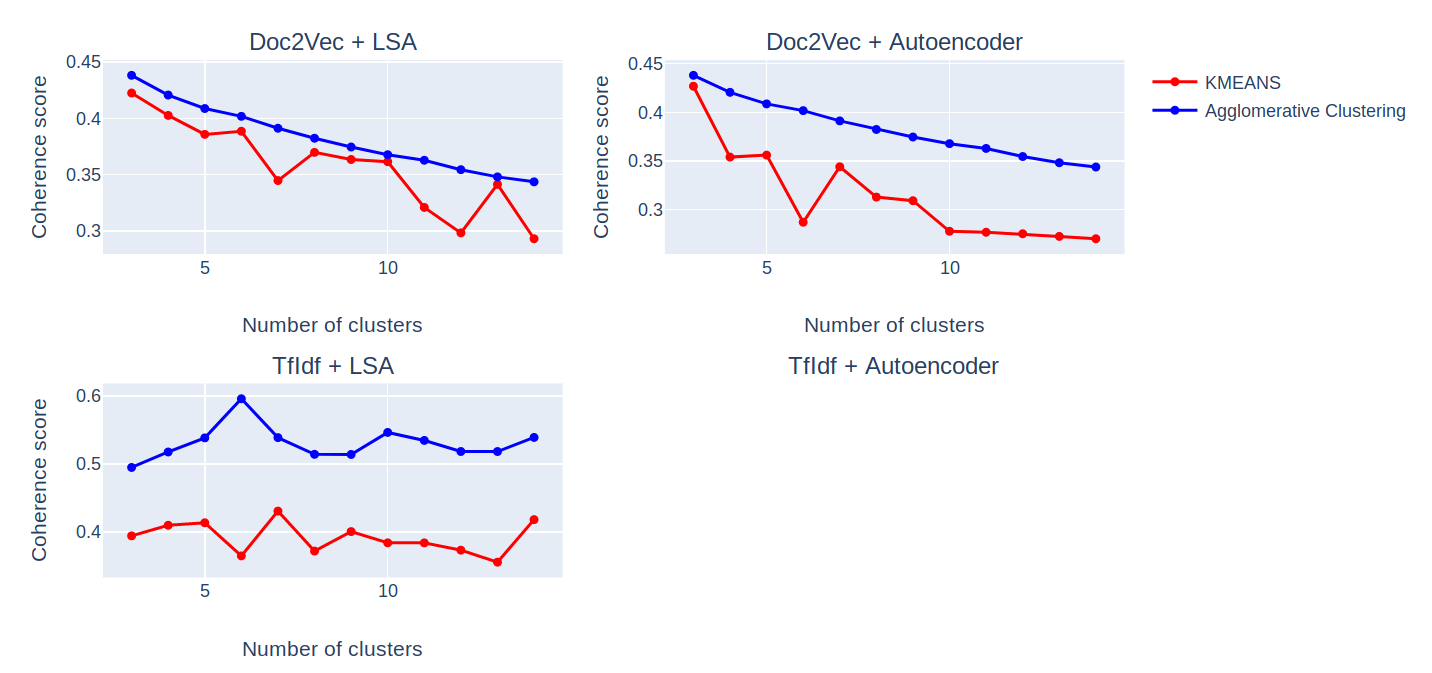
\includegraphics[width=400px]{/home/tim/HCC/IKON-backend/src/topicextraction/nlp/plots/tm_quality}
	\caption{\label{pic:tm_quality} Graph showing the quality of the topic modeling while varying the embedding, topic extraction and clustering model}
\end{figure}

Plotting this combination of models and parameters in \autoref{pic:best_coherence_plot} reveals that there is one huge cluster (cluster 0) while the other 9 clusters contain maximally five projects. A further analysis of the dominating cluster also showed that although its top words suggest projects connected to evolution and biology, there are also a number of projects which deal with geology and paleontology. Interestingly, perturbating the parameters of all models does not change the fact that such a huge cluster forms speaking in favor of the hypothesis that these projects indeed form a huge cluster in the high embedding space.

\begin{figure}[t]
	\centering
	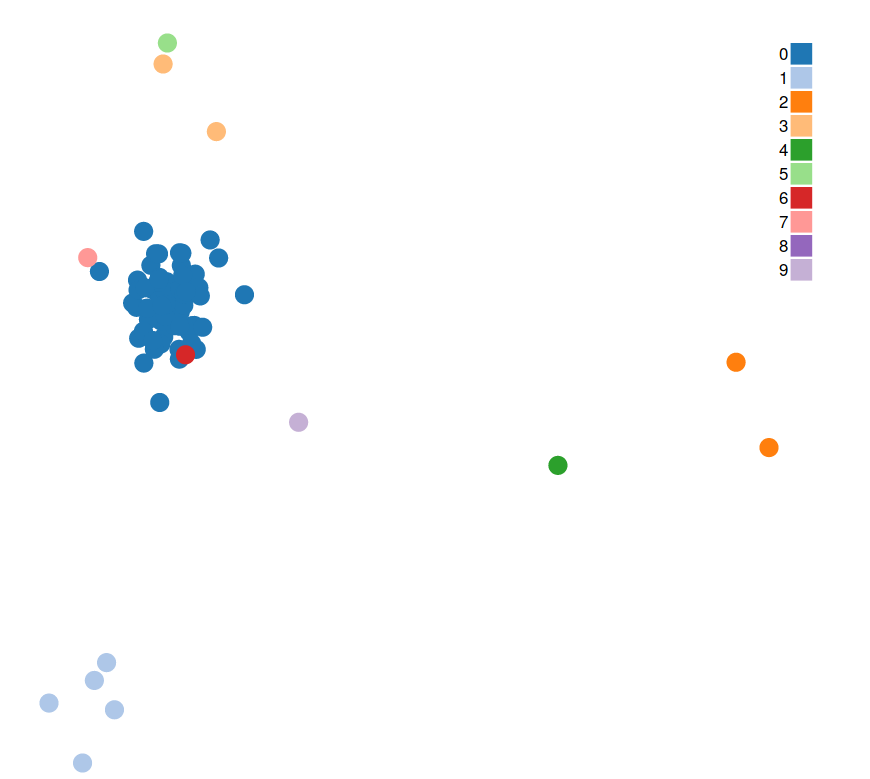
\includegraphics[width=400px]{../chapters/implementation/pics/best_coherence_plot}
	\caption{\label{pic:best_coherence_plot} Plot for the parameter and models with the best coherence score}
\end{figure}

\begin{table}
	\centering
	\begin{tabular}{c | c}
		0 & Datum, Evolution, morphologisch, Taxa, ökologisch \\ \hline
		1 & Sackflügelfledermaus, Abwanderungsverhalten, Weibchen, Männchen, Harem \\ \hline
		2 & Western, Mountains, Kaokoveld, Fauna, Escarpment \\ \hline
		3 & Tansania, biostratigraphische, palynologisch, Tendaguru, Palynologie \\ \hline
		4 & Acentropinae, Philippinen, Trichoptera, Lepidoptera, Reliktendemiten \\ \hline
		5 & SCHRANK, gesichert, Flora, Sauropoden, Gymnospermen \\ \hline
		6 & Praktik, kolonisieren, Mediziner, Gesundheitsbehörden, Malaria \\ \hline
		7 & Magmaozeans, Magmaozean, Planetare, Impaktprozess, Impaktors \\ \hline
		8 & Kurzexpedition, Basilosauridae, Pabdeh, Ablagerungen, Iran \\ \hline
		9 & Hauptexporteur, Kieselalgendiversität, Känozoikum, Silikatverwitterung, Kieselalgen \\ \hline
	\end{tabular}
	\caption{\label{tab:best_coherence_table} Table showing the top words for {\autoref{pic:best_coherence_plot}}}
\end{table}

At this point I gathered feedback from the researchers from project IKON and their answers suggested that problems may occur trying to visualize such dominating structures in scatterplots. \tk{Proper argument?}
Therefore I turned to the second best performing combination of models which is a Doc2Vec embedding, an autoencoder-based topic extraction and a K-Means clustering. The graph also suggests that less clusters improve the quality of the generated top words which I incorporated by constraining the range of selectable numbers of topics.

\section{Reduction into 2D}

\section{Visualization}

In order to visualize all the results from the topic modeling pipeline I developed a D3.js-based interface, which is embedded in the Jupyter notebook in which the code for all the numerical computations resides. Since Jupyter is embracing the browser as a frontend, there is the possibility to embed arbitrary Javascript code in a cell and inject any kind of visualization. In order to do that I construct a JSON object containing all the results from the topic pipeline (vectorized documents as scatter points and linearized points, top words, the interpolated topography, model parameters etc.) and pass it into the Javascript code via Jupyter's $Javascript$ function and string interpolation which renders it in the browser.

\subsection{Explainability technique: Linearization}

As Lipton \cite{liptonMythosModelInterpretability2016a} pointed out, a visualization is already an explainability technique in itself. Therefore we can use the vast amount of interaction design research to optimize the existing interface. 

One of the main problems of scatter graphs is overdrawing, also called clutter. This problem occurs when glyphs are close enough in a scatter plot so that they overlap each other. The higher the density of a region is, the harder it gets to perceive the number of points and the harder it is to annotate the glyphs with additional data \cite{mayorgaSplatterplotsOvercomingOverdraw2013}. 

Normally this problem is hard to solve since the position of points in respect to each other encodes important information. Considering that in this case a high dimensional space is reduced to 2D, there are inherent reduction errors introduced into the distances between points and the absolute distances in 2D loose part of their semantic importance, as discussed in the section concerning the cluster topography. Therefore it is possible to assume that instead of distances, the neighborhood of a point is more important, which leads to the possibility to map the scatter graph on a more regularized structure while preserving the neighborhood of points as well as possible. One way to do so, is to map the points in 2D onto a grid. This problem reduces to a linear assignment problem (LAP), where each point should be assigned to its nearest point in the grid while minimizing the global displacement error. A popular algorithm for that is the Jonker-Volgenant algorithm \cite{jonkerShortestAugmentingPath1987}. Jonker and Volgenant rephrase the LAP as a shortest path problem and by using augmenting paths improve the previously popular Hungarian algorithm to cubic worst-case complexity. 
Applying this to the output of the developed pipeline yields the plots in \autoref{label}.